\begin{exercice}
    Soit $f$ de classe $\mathscr{C}^1$ sur $[a, b]$ telle que $f'$ soit strictement positive sur $[a, b]$. Calculer:
    $$\int_{a}^{b} f(t) \d t + \int_{f(a)}^{f(b)} f^{-1}(t) \d t.$$
\end{exercice}

\begin{elem_sol}
    \begin{itemize}
    \item Comme $f' > 0$, alors $f$ est strictement croissante. De plus, $f$ est continue, donc $f$ réalise une bijection de $[a, b]$ sur $[f(a), f(b)]$.

    \item En effectuant le changement de variable $\phi : [a, b] \to [f(a), f(b)],\, u \mapsto f(u)$, alors $\phi$ est bien de classe $\mathscr{C}^1$ et
    \begin{align*}
    \displaystyle\int_{f(a)}^{f(b)} f^{-1}(t) \mathrm{d} t
    &= \displaystyle\int_a^b f^{-1}(f(u)) f'(u) \mathrm{d} u\\
    &= \displaystyle\int_a^b u f'(u) \mathrm{d} u\\
    &= \left[u f(u)\right]_a^b - \displaystyle\int_a^b f(u) \mathrm{d} u,
    \end{align*}
    où on a effectué une intégration par parties.
    \end{itemize}

    Finalement,
    \[
    \displaystyle\int_a^b f(t) \mathrm{d} t + \displaystyle\int_{f(a)}^{f(b)} f^{-1}(t) \mathrm{d} t = b f(b) - a f(a).
    \]
    
    % \item Calculer le deuxième terme en posant $t = f(u)$.
        % \item Éffectuer une IPP sur le deuxième terme pour conclure. 
        % Donner une interprétation géométrique.
    % \end{itemize}
\end{elem_sol}

\todoinline{Là, il y a un dessin à faire ;-) ! En gros, de mémoire, on peut dessiner un rectangle avec une symétrie par rapport à la première bissectrice. Je vais faire un schéma sur un papier que je mettrai dans le dossier.}

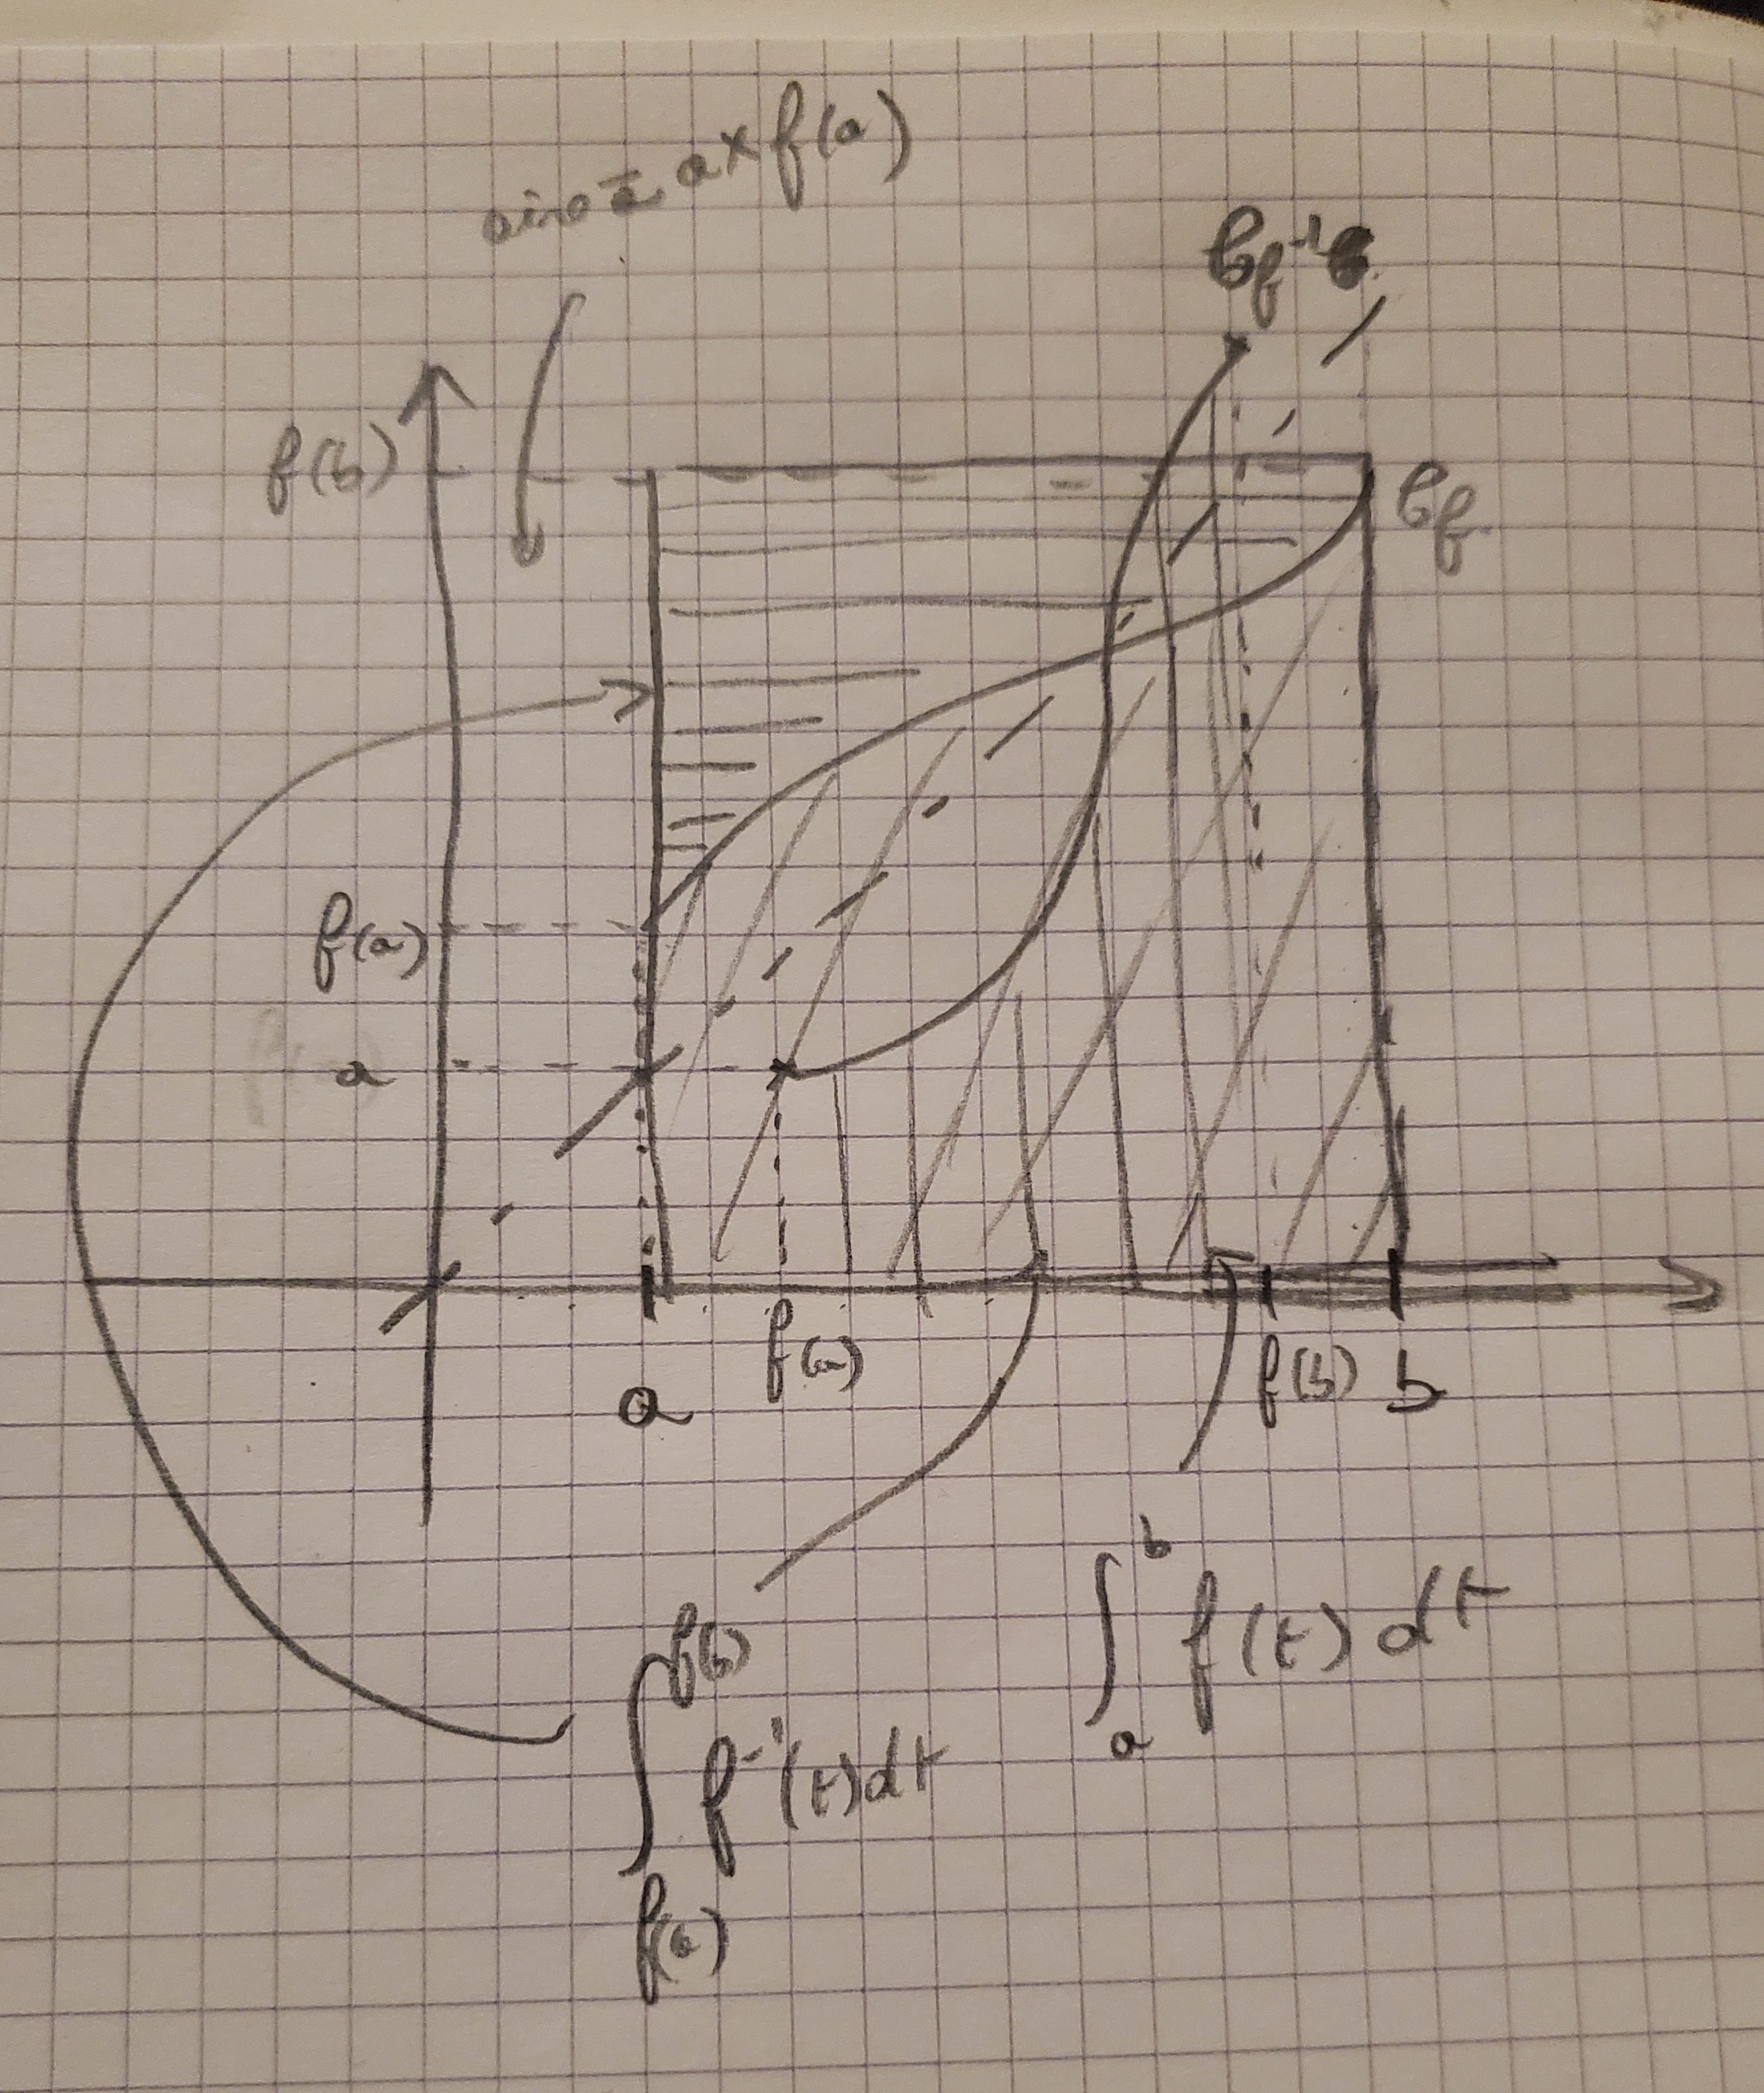
\includegraphics[width=0.5\textwidth]{./chapitres/integration/documents/propriete_geometrique.jpg}